% =====================================================================
%  Chapitre 4 -- partie c : multiclasse, pieges, pratique
% =====================================================================

\begin{frame}{Plus de deux classes : deux stratégies}
\begin{columns}[t]
\begin{column}{0.48\textwidth}
\begin{ebox}[Un contre tous (OvR)]
Un classifieur binaire par classe : « 3 contre le reste », « 8 contre le
reste », « 9 contre le reste ». On garde la probabilité la plus haute.
\end{ebox}
\end{column}
\begin{column}{0.48\textwidth}
\begin{ebox}[Softmax]
Un seul modèle qui produit une distribution sur les $K$ classes :
\[
  \hat p_k=\frac{e^{z_k}}{\sum_{j}e^{z_j}} .
\]
Les probabilités somment à 1.
\end{ebox}
\end{column}
\end{columns}
\vspace{2mm}
\begin{kbox}[Quand cela change quelque chose]
OvR peut donner des scores incohérents (deux classes à 0,7). Le softmax, lui,
arbitre toujours. Pour la régression logistique, scikit-learn utilise OvR par
défaut ; \texttt{multi\_class='multinomial'} passe au softmax.
\end{kbox}
\end{frame}

\begin{frame}{Lire une matrice $3\times3$}
\begin{columns}[t]
\begin{column}{0.44\textwidth}
\centering
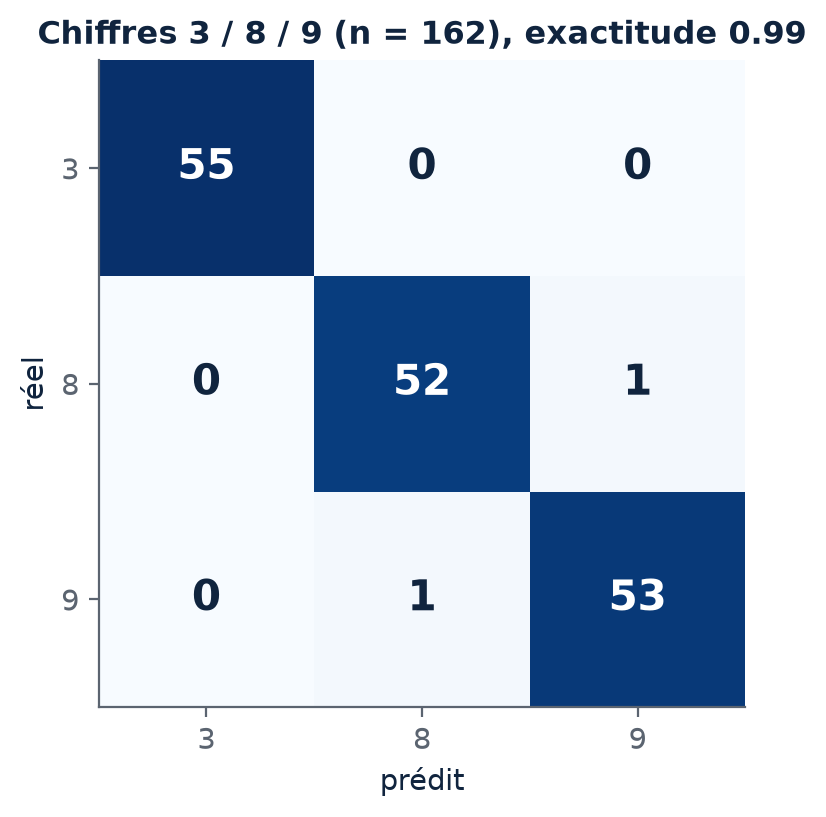
\includegraphics[height=0.31\textheight,keepaspectratio]{l09_multiclasse.png}
\end{column}
\begin{column}{0.54\textwidth}
\begin{itemize}
  \item Chiffres 3, 8 et 9 : exactitude $\mathbf{0{,}988}$.
  \item Rappel par classe : $1{,}000$ / $0{,}981$ / $0{,}981$.
  \item Les erreurs sont \textbf{sur la diagonale adjacente} : 8 confondu avec
        9 et réciproquement.
\end{itemize}
\begin{wbox}[Le réflexe]
Ne jamais lire une matrice $K\times K$ comme un seul chiffre : chercher
\emph{où} sont les erreurs. Ici, le problème est un seul couple de classes.
\end{wbox}
\end{column}
\end{columns}
\end{frame}

\begin{frame}{Macro, micro, pondéré : trois moyennes}
\begin{center}
\small
\begin{tabular}{@{}p{0.16\textwidth}p{0.36\textwidth}p{0.38\textwidth}@{}}
\toprule
\textbf{Moyenne} & \textbf{Calcul} & \textbf{Quand l'utiliser} \\
\midrule
Macro & moyenne des scores par classe & chaque classe compte pareil, même rare \\
Micro & calcul global sur tous les cas & chaque \emph{individu} compte pareil \\
Pondérée & moyenne pondérée par l'effectif & reflète la population réelle \\
\bottomrule
\end{tabular}
\end{center}
\vspace{2mm}
\begin{kbox}[Exemple]
Une classe de 5 individus et une de 500 : la macro donne le même poids aux deux,
la micro est dominée par la grande classe. Un rapport sérieux annonce laquelle
il utilise.
\end{kbox}
\end{frame}

\begin{frame}[fragile]{Le rapport de classification}
\begin{codebox}[Toujours regarder les trois colonnes]
\begin{lstlisting}
from sklearn.metrics import classification_report, confusion_matrix

pred = modele.predict(X_test)
print(confusion_matrix(y_test, pred))
print(classification_report(y_test, pred,
      target_names=["3", "8", "9"], digits=3))
\end{lstlisting}
\end{codebox}
\vspace{1mm}
{\footnotesize
\texttt{precision}, \texttt{recall} et \texttt{f1-score} sont donnés
\textbf{par classe}, puis moyennés. Un $F_1$ global de 0,95 peut cacher une
classe à 0,40.}
\end{frame}

\begin{frame}{Le rapport d'évaluation en six lignes}
\begin{enumerate}
  \item \textbf{Le jeu} : effectif, prévalence, découpage, graine.
  \item \textbf{La référence} : modèle naïf et son score.
  \item \textbf{La matrice de confusion} au seuil retenu.
  \item \textbf{Précision, rappel, $F_1$} --- et l'AUC ou l'AP pour situer.
  \item \textbf{Le seuil et sa justification} (coût, contrainte métier).
  \item \textbf{L'incertitude} : intervalle de confiance ou écart-type sur les plis.
\end{enumerate}
\vspace{1.5mm}
\begin{wbox}[Ce qui manque le plus souvent]
La ligne 2. Sans référence naïve, un score de 0,95 ne veut rien dire : il faut
savoir ce que donne « tout prédire la classe majoritaire ».
\end{wbox}
\end{frame}

\begin{frame}{Le piège du seuil réglé sur le test}
\begin{wbox}[Le scénario]
On essaie 20 seuils sur le jeu de test, on garde celui qui maximise le $F_1$,
puis on annonce ce $F_1$. Le chiffre est \textbf{optimiste} : le seuil a été
choisi en regardant la réponse.
\end{wbox}
\begin{columns}[t]
\begin{column}{0.48\textwidth}
\begin{solbox}[Le protocole correct]
Régler le seuil sur un jeu de \textbf{validation} ou par validation croisée
interne ; n'utiliser le test qu'une fois, avec le seuil figé.
\end{solbox}
\end{column}
\begin{column}{0.48\textwidth}
\begin{kbox}[Combien cela coûte]
Sur 20 seuils testés, l'écart entre le $F_1$ optimiste et le $F_1$ honnête peut
atteindre plusieurs points, surtout avec peu de positifs.
\end{kbox}
\end{column}
\end{columns}
\end{frame}

\begin{frame}{Étude de cas : le modèle à 99 \%}
\begin{abox}[La situation]
Un prestataire annonce 99,2 \% d'exactitude pour prédire l'abandon d'étudiants.
Le jeu contient 4 \% d'abandons. Le rapport ne donne ni précision, ni rappel,
ni matrice, ni seuil.
\end{abox}
\vspace{1mm}
\begin{columns}[t]
\begin{column}{0.48\textwidth}
\begin{enumerate}
  \item Que vaut l'exactitude d'un modèle qui prédit « personne n'abandonne » ?
  \item Que demander en premier ?
  \item Quel usage pédagogique rendrait ce modèle utile ?
\end{enumerate}
\end{column}
\begin{column}{0.48\textwidth}
\begin{solbox}[Réponses]
\textbf{1.} $96$ \%. Le modèle n'apporte que 3 points.
\textbf{2.} La matrice de confusion, le rappel et le seuil.
\textbf{3.} Un rappel élevé pour déclencher un accompagnement, quitte à
convoquer des étudiants qui n'auraient pas décroché.
\end{solbox}
\end{column}
\end{columns}
\end{frame}

\begin{frame}{Activité 3 --- choisir la métrique (10 min)}
\begin{abox}[Quatre situations]
\begin{enumerate}
  \item Filtre anti-spam : un courriel légitime bloqué est très gênant.
  \item Dépistage d'une maladie grave et traitable.
  \item Attribution automatique de mentions (A à F).
  \item Prédiction du décrochage pour cibler un tutorat.
\end{enumerate}
Quelle métrique privilégier, et à quel seuil ?
\end{abox}
\vspace{1mm}
\begin{solbox}[Réponses]
\textbf{1.} Précision (seuil haut). \textbf{2.} Rappel (seuil bas).
\textbf{3.} Exactitude et $F_1$ macro. \textbf{4.} Rappel, avec un seuil réglé
sur le coût d'un tutorat inutile.
\end{solbox}
\end{frame}

\begin{frame}{Quiz 3 --- multiclasse et protocole}
\begin{columns}[t]
\begin{column}{0.49\textwidth}
\begin{qbox}[Question 1]
La moyenne macro :
\begin{itemize}
  \item[(a)] pondère par l'effectif
  \item[(b)] donne le même poids à chaque classe
  \item[(c)] est toujours égale à l'exactitude
\end{itemize}
\end{qbox}
\begin{qbox}[Question 2]
Régler le seuil sur le test :
\begin{itemize}
  \item[(a)] est correct
  \item[(b)] rend le score optimiste
  \item[(c)] améliore la calibration
\end{itemize}
\end{qbox}
\end{column}
\begin{column}{0.49\textwidth}
\begin{qbox}[Question 3]
Le softmax garantit :
\begin{itemize}
  \item[(a)] des probabilités qui somment à 1
  \item[(b)] un rappel élevé
  \item[(c)] la calibration
\end{itemize}
\end{qbox}
\begin{solbox}[Réponses]
\textbf{1.} (b). \quad \textbf{2.} (b). \quad \textbf{3.} (a) seulement.
\end{solbox}
\end{column}
\end{columns}
\end{frame}

\begin{frame}{À retenir et TP}
\begin{kbox}[Les six idées du chapitre]
\begin{enumerate}
  \item Un classifieur produit une probabilité ; le seuil est une décision.
  \item La matrice de confusion est le point de départ, pas le score global.
  \item Précision et rappel s'opposent : le choix dépend du coût des erreurs.
  \item Sur données déséquilibrées, l'exactitude ment ; utiliser PR et le rappel.
  \item L'AUC mesure le classement, pas la qualité au seuil retenu.
  \item Le seuil et les métriques se règlent sur la validation, jamais sur le test.
\end{enumerate}
\end{kbox}
\vspace{1.5mm}
\begin{abox}[TP4 : \file{notebooks/TP4_classification_evaluation.ipynb}]
Comparer un modèle naïf et une régression logistique sur un jeu déséquilibré ;
tracer ROC et PR ; régler le seuil par coût ; mesurer l'effet de la pondération.
Durée : \textbf{3 h} · barème : \textbf{15 points}.
\end{abox}
\end{frame}
